\renewcommand{\labelitemi}{\textsc{\labelitemiv}}

\chapter[Statistica Descrittiva]{Statistica Descrittiva}

\section{Introduzione}

\subsubsection{Statistica Descrittiva, Statistica Inferenziale e Probabilità}

La statistica è l'arte di imparare dai dati. Possiamo suddividerla in:
\begin{itemize}
    \item \textbf{Statistica Descrittiva}: \textit{Descrive} e riassume i dati
    \item \textbf{Statistica Inferenziale}: \textit{Trae} conclusioni dai dati
\end{itemize}
Per poter trarre conclusioni dai dati, bisogna tenere conto del ruolo che gioca il caso. Definiamo quindi la \textbf{probabilità} come la descrizione matematica di eventi \textit{casuali}.

\section{Descrivere i dati}

\subsection{Frequenze, Istogrammi, Classi}

\subsubsection{Frequenza Assoluta e Relativa}

Misuriamo una certa variabile in un campione, ottenendo un insieme di dati. Se i dati non sono distinti, ovvero \textit{abbiamo ripetizioni}, possiamo riassumerli in una \textbf{tabella delle frequenze}. Possiamo definire dunque:

\begin{itemize}
    \item \textbf{Frequenza Assoluta $f_i$ }:= numero di volte in cui i compare nel campione di dati.
    \item \textbf{Frequenza Relativa $p_i$ }:= $\sfrac{f_i}{N}$ = numero di volte in cui compare i rispetto al totale.  
\end{itemize}

\begin{tcolorbox}
    \textbf{Esempio}: Marta intervista i suoi N = 20 compagni di classe e chiede la squadra di calcio preferita, ottenendo le risposte: \newline \textit{Juve, Milan, Inter, Atalanta, Juve, Milan, Nessuna, Nessuna, Inter, Milan, Juve, Nessuna, Atalanta, Juve, Nessuna, Milan, Inter, Milan, Nessuna, Nessuna}. \newline
    
    \begin{tabular}{ |p{3.5cm}|p{3.5cm}|p{3.5cm}|  }
        \hline
        \multicolumn{3}{|c|}{Squadre di Calcio} \\
        \hline
        Valori & Frequenze assolute & Frequenze relative \\
        \hline
        Juve & 4 & 4/20 = 0.20 \\
        Milan & 5 & 5/20 = 0.25 \\
        Inter & 3 & 3/20 = 0.15 \\
        Nessuna & 6 & 6/20 = 0.30 \\
        Atalanta & 2 & 2/20 = 0.10 \\
        \hline
    \end{tabular}
\end{tcolorbox}

\subsubsection{Istogramma}

É utile rappresentare le frequenze mediante un grafico a barre detto \textbf{istogramma}. \newline

\begin{figure}[htbp]
    \centering
    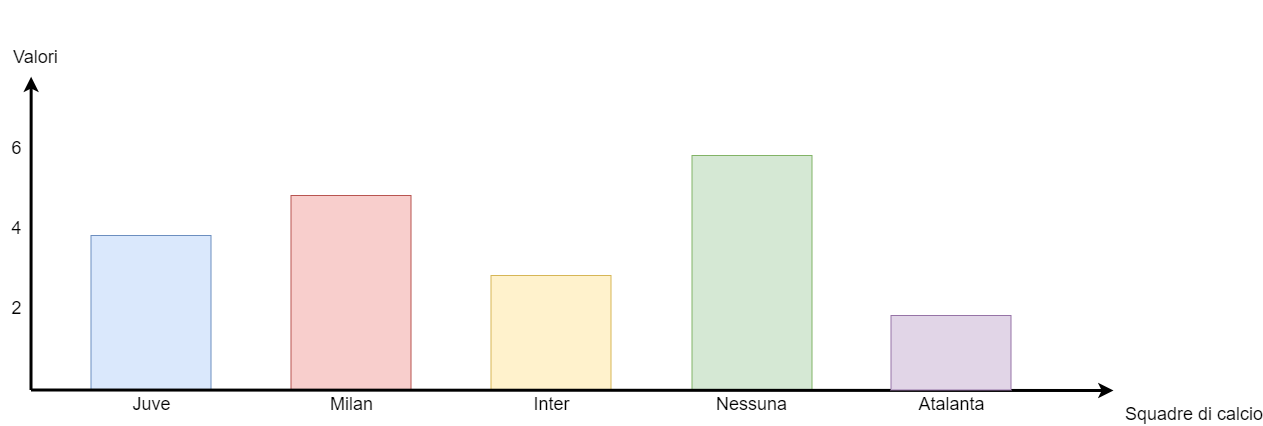
\includegraphics[scale=.4]{Foto/barchart.png}
    \color{gray}
    \caption{Istogramma sulle frequenze assolute delle squadre di calcio} 
\end{figure}

\newpage
\subsubsection{Classi}

Può capitare di avere insiemi di dati che assumono un numero elevato di valori distinti. In tal caso conviene \textit{suddividere} i valori assunti in intervalli detti \textbf{classi}. \newline

\begin{tcolorbox}
\textbf{Esempio}: Vengono misurati i livelli di colesterolo nel sangue di un insieme di N = 40 individui: 
\begin{center}
    213 174 193 796 220 183 194 200 192 200  200 199 178 183 188 193 187 181 193 205 196 211 202 213 216 206 195 191 171 194 184 191 221 212 221 204 204 191 183 227
\end{center}
Molti valori sono distinti e dunque hanno $f_i = 1$. Scegliamo le classi: 
\begin{center}
    ${[170,180) \quad [180,190) \quad [190,200) \quad [200,210) \quad [210,220) \quad [220,230)}$
\end{center}

\begin{tabular}{ |p{3.5cm}|p{3.5cm}|p{3.5cm}|  }
    \hline
    \multicolumn{3}{|c|}{Livelli di colesterolo} \\
    \hline
    Valori & Frequenze assolute & Frequenze relative \\
    \hline
    $[170,180)$ & 3 & 3/40 = 7.5 \\
    $[180,190)$ & 7 & 7/40 = 17.5 \\
    $[190,200)$ & 13 & 13/40 = 32.5 \\
    $[200,210)$ & 8 & 8/40 = 20 \\
    $[210,220)$ & 5 & 5/40 = 12.5 \\
    $[220,230)$ & 4 & 4/40 = 10 \\
    \hline
\end{tabular}
\end{tcolorbox}

\newpage
\subsection{Dati Bivariati}


I \textbf{dati bivariati} ci permettono di mostrare \textit{due variabili} per ogni singolo elemento dell'insieme. Per un elemento i, indichiamo con $x_i$ la prima variabile e con $y_i$ la seconda.

\subsubsection{Diagramma Di Dispersione} 

Un \textbf{diagramma di dispersione} rappresenta i punti ($x_i$, $y_i$), in modo da evidenziare una possibile \textit{correlazione} tra i due valori.\newline

\begin{tcolorbox}
    \textbf{Esempio}: Rileviamo il numero di anni di scuola (prima variabile) e le pulsazioni a riposo (seconda variabile) in un campione di N=10 individui. I dati ($xi$ , $yi$) sono
    \begin{center}
        (12,73) (16,67) (13,74) (18,63) (19,73) (12,84) (18,60) (19,62) (12,76) (14,71)
    \end{center}
    \centering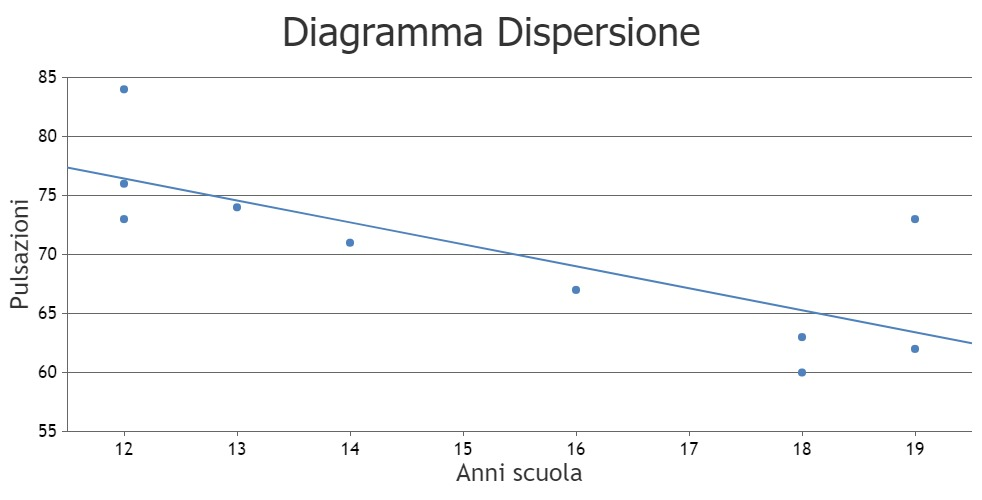
\includegraphics[scale=.3]{Foto/Chart.jpeg} \newline
    Possiamo evidenziare una correlazione negativa tra i due valori.

\end{tcolorbox}

\newpage
\section{Riassumere i dati}

Una \textbf{statistica} campionaria riassume l'insieme di dati mediante una quantità numerica.

\subsection{Indici di Posizione}

Un \textbf{indice di posizione} \textit{sintetizza la posizione} di una distribuzione sostituendo l'insieme dei dati con un unico valore tale da fornire una rappresentazione globale.

\subsubsection{Media Campionaria}

Per definire il valore medio dell'insieme dei dati, definiamo la \textbf{media campionaria} come $$ \overline{x} := \dfrac{x_1 + x_2 + \cdots + x_N}{N} = \dfrac{1}{N} \sum_{i=1}^n x_i $$

\noindent In generale, sapendo le frequenze assolute dei valori, possiamo scrivere la media campionaria come $$ \overline{x} = \dfrac{z_1 \cdot f_1 + z_2 \cdot f_2 + \cdots + z_M \cdot f_M}{N}$$ con $N= f_1 + f_2 + \cdots + f_M$, dove $z_i$ sono i valori e $f_i$ sono le frequenze assolute associate. \newline

\noindent \textbf{Osservazione}: La media è lineare: $\overline{y} = a \cdot \overline{x} + b$ 

\subsubsection{Mediana Campionaria}

Un'altra misura del centro dell'insieme dei dati è la \textbf{mediana campionaria}, ovvero quel valore che, ordinati i dati, si trova in \textit{posizione centrale}. In base al numero di dati, si calcola in due modi:

\begin{itemize}
    \item \textbf{N dispari}: la mediana è il dato di posto $\frac{N+1}{2}$ :  $$ m := x_{\left(\frac{N+1}{2}\right)} $$ 
    \item \textbf{N pari}: la mediana è la media aritmetica tra il dato di posto $\frac{N}{2}$ e quello di posto $\frac{N}{2} + 1$ :  $$ m := \frac{x_{\left(\frac{N}{2} \right)} + x_{\left(\frac{N}{2}+1\right)}}{2} $$
\end{itemize}

\subsubsection{Percentile Campionario}

Fissiamo un numero $ k \in [0, 100]$. Definiamo il \textbf{k-esimo percentile campionario} il valore t per cui:
\begin{itemize}
    \item almeno il $k\%$ dei dati è $\leq$ t
    \item almeno il $(100-k)\%$ dei dati è $\geq$ t
\end{itemize}

\subsubsection{Quartili}

I casi più importanti sono:
\begin{itemize}
    \item \textbf{Primo Quartile} $q_1$: $p = \dfrac{1}{4}$, $k=100p$
    \item \textbf{Secondo Quartile} $q_2$: $p = \dfrac{1}{2}$, $k=100p$
    \item \textbf{Terzo Quartile} $q_3$: $p = \dfrac{3}{4}$, $k=100p$
\end{itemize}

\noindent Come per la mediana, si calcola in due modi:
\begin{itemize}
    \item Se $N \cdot p$ non è intero, $t=x_{(i)}$ è il dato di posizione i definito come l'intero successivo a $N \cdot p$
    \item Se $N \cdot p$ è intero, $t= \dfrac{x_{(N \cdot p)} + x_{(N\cdot p+1)}}{2}$
\end{itemize}

\begin{tcolorbox}
    \textbf{Esempio}: Ai 1000 abitanti di un piccolo comune viene chiesto di esprimere un giudizio su un nuovo servizio comunale, usando una scala da 0 a 4. 251 persone hanno votato 0, 260 persone hanno votato 1, 80 persone hanno votato 2, 154 persone hyanno votato 3 mentre 255 persone hanno votato 4\newline
    Vogliamo calcolare i 3 indici di posizione: Media, Mediana, Quartili. \newline
    \begin{itemize}
        \item \textbf{Media}: $\overline{x} = \dfrac{0 \cdot 251 + 1 \cdot 260 + 2 \cdot 80 + 3 \cdot 154 + 4 \cdot 255}{1000}= 1,902 \simeq 1,9$
        \item \textbf{Mediana}: $m = \dfrac{x_{(500)} + x_{(501)}}{2} = \dfrac{1+1}{2}= 1$
        \item \textbf{Primo quartile}: $1000 \cdot \dfrac{1}{4} = 250 $, $q_1 = \dfrac{x_{(250)} + x_{(251)}}{2} = \dfrac{0+0}{2}=0$
        \item \textbf{Secondo quartile}: mediana = 1
        \item \textbf{Terzo quartile}: $ 1000 \cdot \dfrac{3}{4} = 750 $, $q_3 = \dfrac{x_{(750)} + x_{(751)}}{2} = \dfrac{4+4}{2}=4$
    \end{itemize}
\end{tcolorbox} 

\subsubsection{Box Plot}

Una rappresentazione grafica di mediana e quartili viene fornita dal \textbf{box plot}:
\begin{figure}[h!]
    \centering
    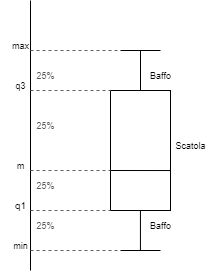
\includegraphics[scale=.6]{Foto/baba.png}
\end{figure}

\subsection{Indici di Dispersione}

Un \textbf{indice di dispersione} descrive la \textit{variabilità di distribuzione} quantitativa dei dati, ovvero quanto i valori presenti distano da un valore centrale.  

\subsubsection{Scarti}

Gli \textbf{scarti} sono la distanza di ogni singolo elemento dal valore medio. La somma di tutti gli scarti è nulla. $$w:= (x_i - \overline{x})$$ 

\subsubsection{Varianza Campionaria}

Considerando gli scarti elevati al quadrato e facendone una sorta di media, otteniamo la \textbf{varianza campionaria} come: $$ s^2 := \dfrac{1}{N-1} \sum_{i=1}^N(x_i - \overline{x})^2 $$ 

\subsubsection{Deviazione Standard}

Per ottenere una statistica omogenea ai dati, si definisce \textbf{deviazione standard} come: $$ s := \sqrt{s^2} = \sqrt{\dfrac{1}{N-1} \sum_{i=1}^N(x_i - \overline{x})^2}$$ 

\subsubsection{Scarto Interquartile}

Un altro indicatore di dispersione rispetto alla mediana m è lo \textbf{scarto interquartile}. Per costruzione, questo intervallo contiene almeno il 50\% dei dati. Il suo valore è: $$ IQR = \Delta := q_3 - q_1$$  \newline

\noindent \textbf{Osservazione}: La varianza e la deviazione standard non sono lineari. \newline 

%\noindent \textbf{Teorema}: L'intervallo attorno a $\overline{x}$ di ampiezza proporzionale a $s$: $$(\overline{x} - c \cdot s, \overline{x} + c \cdot s) \qquad c \geq 0$$ contiene una frazione di dati pari a: $$\alpha \geq 1 - \dfrac{1}{c^2} $$ Ad esempio, se c=2, avremo il 75\% dei dati nell'intorno, con c=3 avremo l'89\%.% 

\subsection{Correlazione}

Consideriamo un insieme di dati bivariati. Vogliamo quantificare la correlazione tra le due variabili x e y, ossia la \textit{tendenza} per cui a valori di x grandi corrispondo valori di y grandi o piccoli. Definiamo quindi il \textbf{coefficiente di correlazione lineare}: $$r =  \dfrac{ \sum_{i=1}^N (x_i-\overline{x})(y_i - \overline{y})}{(N-1)\cdot s_x \cdot s_y} \quad \text{oppure} \quad r =  \dfrac{ \sum_{i=1}^N x_i \cdot y_i - N \cdot \overline{x} \cdot \overline{y}}{(N-1)\cdot s_x \cdot s_y}$$  Il coefficiente di correlazione lineare può assumere valori $\in [-1, 1]$. Nello specifico diremo che:
\begin{itemize}
    \item $|r| \gtrsim 0,7$ avremo correlazione \textit{significativa}
    \item $|r| \lesssim 0,3$ avremo correlazione \textit{debole}.
\end{itemize} 

\begin{tcolorbox}
    \textbf{Esercizio Completo}: Prendiamo un campione di N = 10 elementi e assegnamo x = numero anni di scuola e y = pulsazioni. Otteniamo i seguenti valori 
    \begin{center}
        (12, 73) (16, 67) (13, 74) (18, 63) (19, 73) (12, 84) (18, 60) (19, 62) (12, 76) (14, 71)
    \end{center}
    Calcoliamo $\overline{x}, m, s^2, s, r$.
    \begin{itemize}
        \item $\overline{x} = \frac{12 + 16 + 13 + 18 + 19 + 19 + 12 + 18 + 19 + 12 + 14}{10} = 15,3$
        \item $s_{x}^2 = \frac{(12 + 16 + 13 + 18 + 19 + 19 + 12 + 18 + 19 + 12 + 14)^2 - 10 \cdot (15,3)^2}{9} \simeq 9,12$
        \item $s_x = \sqrt{s_{x}^2} \simeq 3,02 $
        \item $\overline{y} = \frac{73 + 67 + 74 + 63 + 73 + 84 + 60 + 62 + 76 + 71}{10} = 70,3$
        \item $s_{y}^2 = \frac{(73 + 67 + 74 + 63 + 73 + 84 + 60 + 62 + 76 + 71)^2 - 10 \cdot (70,3)^2}{9} \simeq 54,23$
        \item $s_y = \sqrt{s_{y}^2} \simeq 7,36 $
        \item $ \dsum_{i=1}^N x_i \cdot y_i = 12 \cdot 73 + 16 \cdot 67 + 13 \cdot 74 + \cdots + 14 \cdot 71 = 10603$
        \item $ r = \frac{10603 - 10 \cdot 15,3 \cdot 70,3}{9 \cdot 3,02 \cdot 7,36} \simeq -0,76$
    \end{itemize}
    Il valore di r conferma che x e y mostrano una significativa correlazione negativa
\end{tcolorbox} 




    